\documentclass[]{article}
\usepackage[spanish]{babel}
\usepackage{graphicx}
\usepackage{xcolor}
\usepackage[utf8]{inputenc}
\usepackage{fancyhdr}
\usepackage{lastpage}
\usepackage{enumitem}
\usepackage{listings}
\usepackage{float}
\usepackage{verbatim}
\usepackage{verbatimbox}
\usepackage{booktabs}
\usepackage{makecell}
\usepackage{tabularx}

\pagestyle{fancy}
\fancyhf{}
\rfoot{Page \thepage\hspace{1pt} de~\pageref{LastPage}}

\title{Proyecto de Redes de Computadores}
\author{Guillermo López García
\and
Gonzalo Ulibarri García
\and
Félix Lázaro Palacio
\and
Alfredo Ramos García
\and
Santiago Jesús Mas Peña
\and
\ldots
\and
\ldots
\and
\ldots
}

\begin{document}
\maketitle
\newpage

\section{Primera Hoja}
\begin{table}[h!]
  \begin{center}
    \caption{Preguntas Integrantes}
    \begin{tabular}{ccccc}
      \toprule
      \textbf{Integrantes} & \textbf{Pregunta 1} & \textbf{Pregunta 2}
      \textbf{Pregunta 3} & \textbf{Pregunta 4} \\
      \midrule
      1 &  &  \\
      2 &  &  \\
      3 &  &  \\
      4 &  &  \\
      5 &  &  \\
      6 &  &  \\
      7 &  &  \\
      8 &  &  \\
      \bottomrule
    \end{tabular}
  \end{center}
\end{table}

\begin{table}[h!]
  \begin{center}
    \caption{Preguntas Integrantes}
    \begin{tabular}{ccccc}
      \toprule
      \textbf{Integrantes} & \textbf{Pregunta 5} & \textbf{Pregunta 6}
      \textbf{Pregunta 7} & \textbf{Pregunta 8} \\
      \midrule
      1 &  &  \\
      2 &  &  \\
      3 &  &  \\
      4 &  &  \\
      5 &  &  \\
      6 &  &  \\
      7 &  &  \\
      8 &  &  \\
      \bottomrule
    \end{tabular}
  \end{center}
\end{table}

\textbf{Coordinador/a: } Guillermo López García. \newline
\textbf{Ponente 1: } Guillermo López García. \newline
\textbf{Ponente 2: } Gonzalo Ulibarri García.
\\
\\
\underline{Pregunta 1:} \\
\underline{Pregunta 2:} \\
\underline{Pregunta 3:} \\
\underline{Pregunta 4:} \\
\underline{Pregunta 5:} \\
\underline{Pregunta 6:} \\
\underline{Pregunta 7:} \\
\underline{Pregunta 8:} \\

\newpage

\section{Segunda Hoja}
\begin{table}[h!]
  \centering
  \begin{center}
    \caption{Tabla profesor}
    \resizebox{\columnwidth}{!}{
        \begin{tabular}{ccc}
          \toprule
          \textbf{Conceptos a valorar} & \textbf{Puntuación Máxima} & \textbf{Puntuación Otorgada} \\
          \midrule
          Contenido del dossier claro y detallado & 3 puntos &  \\
          \midrule
          Maquetación/Formato del dossier         & 1 punto  &  \\
          \midrule
          Ponente 1                               & 1 punto  &  \\
          \midrule
          Ponente 2                               & 1 punto  &  \\
          \midrule
          Preguntas formuladas                    & 4 puntos &  \\
          \midrule
          Puntuación total                        & \multicolumn{2}{c}{} \\
          \bottomrule
        \end{tabular}
    }
  \end{center}
\end{table}

\newpage

\tableofcontents

\newpage

\section{Documento 1: Planos de Cableado Horizontal}
	\begin{center}
    \centering
    \textbf{
        {\large En plano anexo.}
   	}
	\end{center}

\newpage

\section{Documento 2: Distribuidores}
\begin{table}[ht!]
  \centering
  \begin{center}
    \caption{Tabla distribuidores 1}
    \resizebox{\columnwidth}{!}{
        \begin{tabular}{ccccccccc}
          \toprule
          \multicolumn{3}{l}{Etiqueta del distribuidor: A- } & \multicolumn{2}{c}{} \\
          \midrule
          \multicolumn{3}{l}{Altura mínima del distribuidor: 27U } & \multicolumn{2}{c}{} \\
          \midrule
          \multicolumn{3}{l}{Ubicación: Primera planta } & \multicolumn{2}{c}{} \\
          \midrule
          \textbf{Dispositivo} & \textbf{Capa OSI} & \textbf{Altura} &
          \textbf{Nº Puertos} & \textbf{Estándar*} & \textbf{TAT Etiquetas*} &
          \textbf{Tipo Conector} & \textbf{Categoría} & \textbf{Cantidad} \\
          \midrule
          Switch Fibra & Enlace & 1U & 48 PoE / 4 SFP & IEEE 802 & RJA1-RJA132(Fija --- Datos) PAA1-PAA7 & GG45 / RJ45 / LC & 4 & 4 \\
          \midrule
          Punto de Acceso & Enlace & --- & 1 PoE & IEEE 802.3af & PAA1-PAA7 & RJ45 & 7 & 7 \\
          \midrule
          Path Panel Datos/VoIP/Wifi & Física & 2U & 48 & --- & RJA1-RJA132(Fija --- Datos) PAA1-PAA7 & GG45/RJ45 & --- & 4 \\
          \midrule
           &  &  \\
          \midrule
           & \multicolumn{2}{c}{} \\
          \bottomrule
        \end{tabular}:
    }
  \end{center}
\end{table}

\begin{table}[ht!]
  \centering
  \begin{center}
    \caption{Tabla distribuidores 2}
    \resizebox{\columnwidth}{!}{
        \begin{tabular}{ccccccccc}
          \toprule
          \multicolumn{3}{l}{Etiqueta del distribuidor: B- } & \multicolumn{2}{c}{} \\
          \midrule
          \multicolumn{3}{l}{Altura mínima del distribuidor: 27U } & \multicolumn{2}{c}{} \\
          \midrule
          \multicolumn{3}{l}{Ubicación: Planta baja } & \multicolumn{2}{c}{} \\
          \midrule
          \textbf{Dispositivo} & \textbf{Capa OSI} & \textbf{Altura} &
          \textbf{Nº Puertos} & \textbf{Estándar*} & \textbf{TAT Etiquetas*} &
          \textbf{Tipo Conector} & \textbf{Categoría} & \textbf{Cantidad} \\
          \midrule
          Router & Red & 1U & 2GE/n4\---10GE/2 SFP  & IEEE 1588 & --- & GG45 / RJ45 / LC & 7 & 1 \\
          \midrule
          Switch Fibra & Enlace & 1U & 48 PoE / 4 SFP & IEEE 802 & RJB1-RJB232(Fija --- Datos) PAB1-PAB7 & GG45 / RJ45 / LC & 6 & 6 \\
          \midrule
          Punto de Acceso & Enlace & --- & 1 PoE & IEEE 802.3af & PAB1-PAB7 & RJ45 & 7 & 7 \\
          \midrule
          Path Panel Datos/VoIP/Wifi & Física & 2U & 48 & --- & RJB1-RJB232(Fija --- Datos) PAB1-PAB7 & GG45/RJ45 & --- & 6 \\
          \midrule
          Path Panel Fibra & Física & 2U & 6 & --- & FB1 --- FB6(Multimode VDSL/ADSL+) & LC & --- & 1 \\
          \midrule
          Dispositivo Firewall & Transporte & 1U & 7 (5 + 2 USB) & --- & --- & RJ45 / USB & --- & 1 \\
          \midrule
           &  &  \\
          \midrule
           &  &  \\
          \midrule
           & \multicolumn{2}{c}{} \\
          \bottomrule
        \end{tabular}
    }
  \end{center}
\end{table}

\begin{table}[ht!]
  \centering
  \begin{center}
    \caption{Direccionamiento Planta Alta y Baja}
    \resizebox{\columnwidth}{!}{
        \begin{tabular}{cc}
          \toprule
          \textbf{Planta A} \\
          \midrule
          \textbf{Elemento} & \textbf{Dirección IP} \\
          \midrule
          VLAN Switch 1 --- VLAN Switch 4 & 172.20.0.2/22 --- 172.20.0.5/22 \\
          RJA1 --- RJA132 (Fija --- Datos) & 172.20.0.6/22 --- 172.20.0.137/22 \\
          \midrule
          Punto de Acceso (Etiquetas) \\
          PAA1 --- PAA7 & 172.20.0.138/22 --- 172.20.0.144/22 \\
          \midrule
          \textbf{Planta B} \\
          \midrule
          VLAN Switch 1 --- VLAN Switch 6 & 172.20.2.2/22 --- 172.20.2.5/22 \\
          RJB1 --- RJB132 (Fija --- Datos) & 172.20.2.6/22 --- 172.20.2.237/22 \\
          \midrule
          Router: \\
          IP Privada: & 172.20.2.1/22 \\
          IP Pública: & 100.80.10.1/24 \\
          \midrule
          Punto de Acceso (Etiquetas) \\
          PAB1 --- PAB7 & 172.20.2.238/22 --- 172.20.2.244/22 \\
          \bottomrule
        \end{tabular}
    }
  \end{center}
\end{table}

\newpage

\section{Documento 3: Plano de Cableado Vertical}

\newpage

\section{Documento 4: Plano de Conexión de Distribuidores}
\begin{figure}[H]
\centering
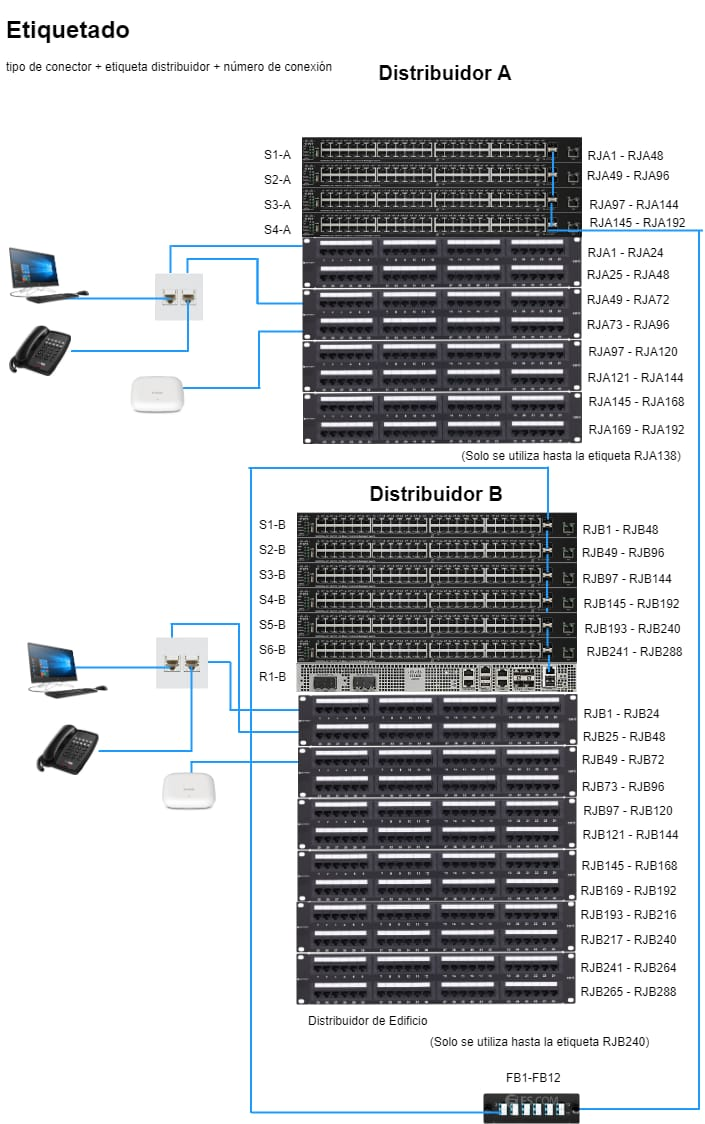
\includegraphics[scale=0.40]{d4}
\caption{}
\end{figure}

%\begin{figure}[H]
%\centering
%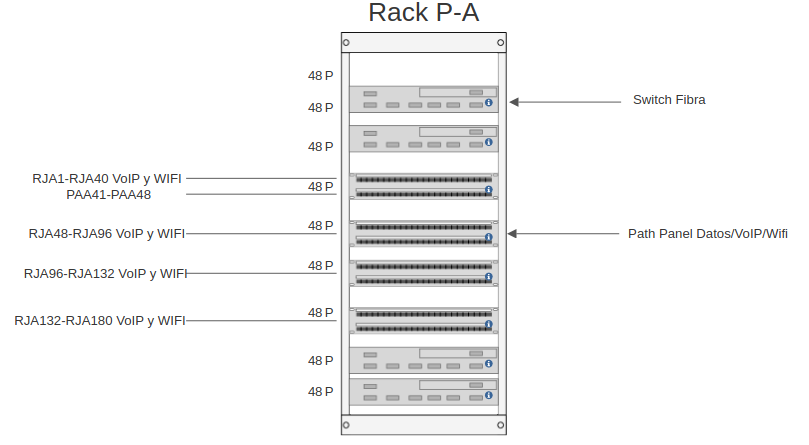
\includegraphics[scale=0.40]{rpa}
%\caption{}
%\end{figure}

%\begin{figure}[H]
%\centering
%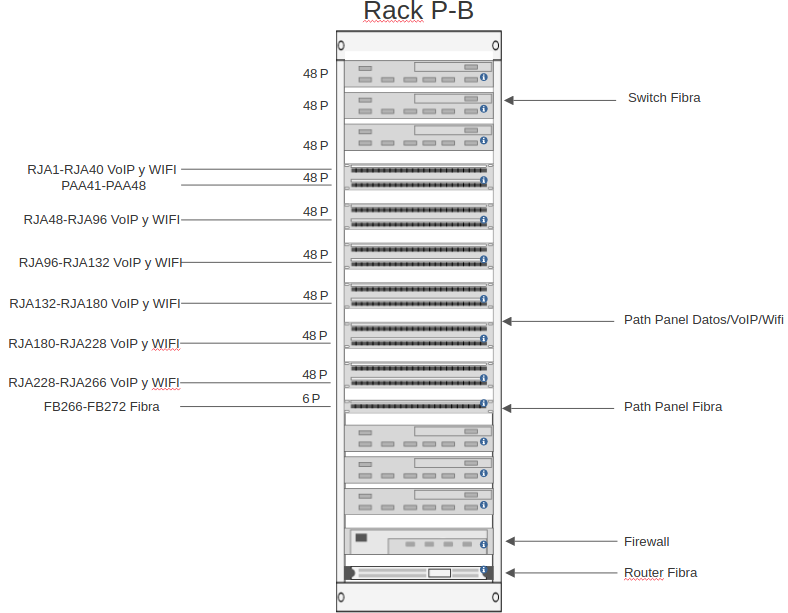
\includegraphics[scale=0.40]{rpb}
%\caption{}
%\end{figure}

\newpage

\section{Documento 5: Justificación}

\begin{enumerate}[label=\alph*]
   \item \underline{Respecto al Documento 1}:
	Respecto al cableado horizontal, se han instalado tomas de conexiones de tamaño específico para cada posible puesto de trabajo. El número de conexiones varía atendiendo al número de dispositivos máximos conectados simultáneamente que se tenga previsto. Se ha considerado también añadir tomas de conexiones para posibles puntos de acceso que cubran toda la superficie del edificio, colocándolas en punto estratégicos que cumplan este requisito. Las tomas dedicadas para los puntos de acceso tendrán únicamente un puerto para estos. \\
	Para los racks, se ha  considerado como buena localización en la planta baja el espacio bajo la escalera hacia la primera planta, y en ésta, la denominada `sala de informática', ya que probablemente en esta sala se encuentren más racks para uso como servidor de datos o para lo que sea pertinente. \\
	La distribución del cableado horizontal se ha pensado para que sea lo más centralizada posible, recorriendo el hall del edificio y manteniendo distancias no muy prolongadas entre las tomas de conexiones y el cableado del hall, permitiendo así que con un único rack por planta ésta quede cubierta.
   \item \underline{Respecto al Documento 2}:
        Hemos considerado la interconexión entre los switches con fibra óptica para aumentar el rendimiento y la velocidad. Cada switch de cada planta irá conectado con fibra multimodo al siguiente switch del respectivo rack. Cada switch del rack A irá conectado al siguiente switch de dicho rack a través de fibra multimodo hasta que llegue al ultimo, entonces, a través del cableado vertical se conecta dicho switch con el primer switch del rack B. Al igual, dichos switch del rack B se conectarán con el siguiente hasta llegar al ultimo, el cual, se conectará con el router.No haremos distinciones entre conexiones, ya sean para voz o datos. \\
        Pensamos además conectar los puntos de acceso con Power Ethernet (PoE) para darle un suministro de energía a dicho dispositivos. \\
        Para las etiquetas, hemos realizado una codificación simple, separando solamente las etiquetas correspondientes a los puntos de acceso. Dicha codificación será:
        \begin{center} (tipo de conector) (etiq distribuidor) (número de conexión)\end{center}
        \begin{center}Ejemplo: RJA4 (conexión 4, planta superior datos / VoIP)\end{center}
        Para el routing, utilizaremos solo un router en el Rack B (Planta Baja). Esto es debido a que no es necesario amplificar la señal de las conexiones mas lejanas, ya que, en ningún caso superara los 100 metros.

   \item \underline{Respecto al Documento 3}: Se ha realizado un plano de la sección vértical 1/2 - G/A. Se han suprimido las vistas de las habitaciones intermedias y los elementos superfluos para realizar un plano simple y preciso. \\
       Hemos realizado el cableado vértical a través del suelo de la primera planta y el falso techo de la segunda planta. Desde el Rack A, hemos dirigido la fibra a través de una canalizaciones en el suelo perpendicular al plano, luego, desde una loseta hemos tirado el cable de fibra multimodo al falso techo de la planta B para dirigirlo hacia la sección del Rack B. Ya en la sección del Rack B, sacamos la fibra a través de una canalización cercana a la escalera, para sacarla del falso techo y unirla al Rack. \\
       Se ha dibujado la fibra multimodo en color verde.
   \item \underline{Respecto al Documento 4}: Respecto al Rack de la Planta A, se ha optado por poner el path panel abajo de los swith para mayor facilidad a la hora de cambiar cableado por algun tipo de error o que se quiera escalabilidad. \\
       Respecto al Rack de la Planta B, se ha optado por la misma decisión, excepto poniendo el router en entre los switch y el path panel. Esto se ha puesto así para que estuviera el router a media altura, y en caso de tener que cambiarlo, para hacer de manera más sencilla y segura. \\
       Además, como se puede ver, en cada path panel hay conexiones hacia las tomas de los puestos de trabajo, tanto para puntos de acceso, VoIP y datos, para los host que trabajen con datos como ordenadores.
   \item \underline{Conclusión Final}: A la conclusión final a la que hemos llegado es que el idear el clabeado, tanto vertical como horizontal, ha sido de lo mas complicado. Sobre todo, a la hora de que se tenía que respetar decisiones de arquitectura y no podiamos campar a nuestras anchas.\\
    Por otro lado, la gestión de distribuidores ha sido más liviana gracias a la información proporcionada por la web de distintas empresas que ofrecen productos con una larga y muy buena especificación. Gracias a ellos, hemos podido saber que es lo que necesitabamos de forma general para que nuestro proyecto de cableado fuera eficaz y simple.\\
    Por último, solo aclarar que la decisión más complicada ha sido la de el plano de conexión en el documento 4, donde, realmente hemos tenido dolores de cabeza para ponerlo de forma idónea para que otros administradores de redes de computadores lo tuvieran lo más fácil posible a la hora de cambiar, disminuir o aumentar el número de swith, path panel y demás componentes que forma parte de este proyecto.
    \item \underline{Historico de realización del proyecto}: \verbfilenobox[\tiny]{historico.txt }
\end{enumerate}

% Para listar fragmentos de codigo de un lenguaje de programacion
% \lstset{language=, texcl=true}
% \begin{lstlisting}[frame=single]
% \end{lstlisting}

% Para listar una secuencia de elementos
% \textbf{}
% \begin{enumerate}
    % \item
% \end{enumerate}

% Para mostrar una figura
% \begin{figure}[H]
% \centering
% \includegraphics[width=0.7\linewidth]{}
% \caption{}
% \end{figure}

% Para listar el contenido de un archivo de texto
% \verbatiminput{.txt}

\end{document}
